\section{Additional findings around Migovec}

\subsection{An overview of surface exploration}

Exploration on the western edge of the plateau has yielded several caves that have piqued our interest in recent years. For instance the JSPDT has concentrated on exploring \passage{Monatip} in the interims between summer expeditions, and every year draws closer to a connection with \passage{System Migovec} at the -100m level. This is both a main aim and hope of our expedition. New caves in the west of the plateau could plausibly connect with \passage[cave]{Primadona}, extending its length and providing new entrances to the system.

In 2014 surface bashing of caves re-discovered in last year’s surface bashing was the focus for western-plateau exploration.

\begin{marginfigure}
\checkoddpage \ifoddpage \forcerectofloat \else \forceversofloat \fi
\centering
\frame{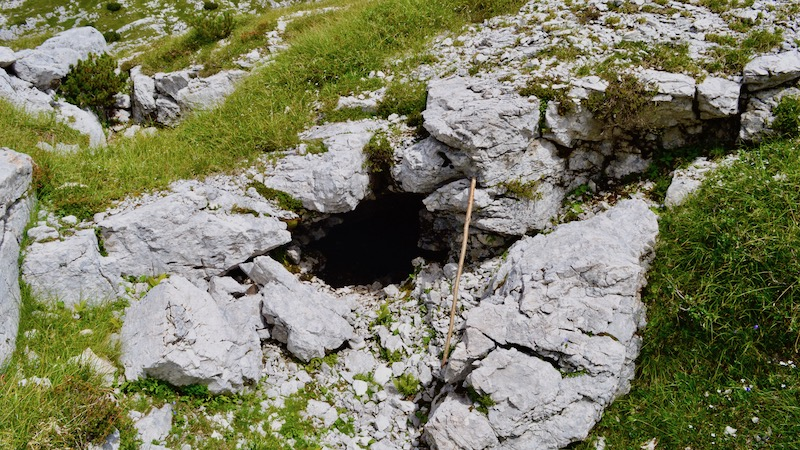
\includegraphics[width=0.99\textwidth]{images/2014/other-finds-2014/n09_tanguy.jpg}}
\caption{The entrance to \passage[entrance]{N09}  was one of the objectives of this year's exploration but the team charged with its relocation lacked a GPS with curated data. This went to highlight the need for a well-managed  and up to date repository of cave location and information --- Tanguy Racine}
\label{end of expo}
\end{marginfigure}

An afternoon of pushing in last year’s main surface discovery, \passage[cave]{Jailbreak}, unfortunately succeeded in killing the cave, as both leads – a dig and a pit containing a boulder blocking onward progression – died. The trip featured a lucky escape for Rhys, the first of a couple he suffered this year!

\passage[dig]{B10}, first marked with red paint during the ‘Blowing Holes Recce’ of 1995, had been looked at in 2013. Located just off the path to \passage[mountain]{Kuk} about 10 minutes from the bivi, it contains a skinny-caver-sized tube suitable for digging with an enlargement referred to as a small chamber. Digging this year expanded the size of the crawling passage, allowing larger cavers to successfully reach the ‘chamber’. The cave continues and \passage[dig]{B10} has potential to reach a length of 10m; however, such gains will only be made with significant digging effort. 

While looking at \passage[dig]{B10} a pit marked as \passage{N01}, shown on various maps of the plateau (and not related to \passage[prospecting region]{Area N} beyond \passage[mountain]{Kuk}), was rediscovered nearby. There was little information about \passage{N01} in the Hollow Mountain despite its presence on maps. A team looked in the bottom of the pit, approximately 3m deep. A tight rift-like wall could conceivably be hammered to reach a small chamber, but there is no visible downward progression. 

A small hole was identified off the path up to the camp and logged as \passage[cave]{Sunset Hole} in the GPS. There is also a rumour of a blowing hole on the scree-slopes approaching the portal (where the paths to \passage[mountain]{Kuk} and \passage[|see{Tolminksi Migovec}]{Migovec} meet and join the path to Tolminski Ravne).


Our re-investigation of \passage[cave]{N1} and logging of small holes such as Sunset Hole ties in with our aim to gain a greater understanding of the plateau. Our current understanding is largely dependent on the experiences of whichever members found/explored each cave entrance.

This ‘scattering’ of mental knowledge makes it difficult to know whether a hole has been previously discovered, killed, or left as a viable lead. We hope to gather together all information about surface cave entrances into one accessible written form within the next few years.

\name{Fiona Hartley}

\subsection{Pushing Balamory to another deep sump}

Following the lead in \passage{Pick Your Poison} that Clare and Grega Maffi had pushed in 2013, Clare convinced Tetley to push the storming passage early in the expedition. At the bottom of \passage{Clapton Pitch}, a large rift with several inlets of water joining in.  Although the leads were not as plentiful as promised (the parallel shaft that beckoned on the survey was a subsidiary to \passage{Clapton}, some significant progress was made. By playing the traverse game, and surviving a brief attack of the ‘Fear', the pair managed to drop another 50m high above the water. Eventually, they returned to stream level, leaving an open, steep descending cascade. This was \passage{Rock Steady Love}.

Later, Grega Maffi and Iztok Mozir pushed the cascade down to 'minus 1000m'. Their efforts were rewarded with a modest, but beautiful sump lake, \passage[sump]{Aja!} at -967m. On their second day at camp, the pair surveyed the passage and derigged the lower section. It was yet another dead end, short of the magic kilometre!


\begin{figure*}[h]
\checkoddpage \ifoddpage \forcerectofloat \else \forceversofloat \fi
\begin{tikzpicture}
\node [name-dest] (box){%
    \begin{minipage}{\textwidth}
    \begin{multicols}{2}
'An interesting trip yesterday. \passage{Clapton} pitch wasn’t quite how Clare remembered it. The two halves of the pitch actually meet at the bottom – as we discovered after 3 bolts. \passage{Pick your Poison} is actually a large stream passage – and due to the rain outside there was a lot of water. We therefore rigged (dry) pitches in places where Maffi and Clare had freeclimbed the last year. At the limit of exploration the streamway is very tight but we found a muddy bypass high in the rift. We left a 15m pitch down to stream level -  named \passage[deep]{Hanging Gardens}.  It’s only 50m in the book but soon we’ll return to drop this pitch. Hopefully we’ll find nice wide stream passage.'
\name{Tetley}

 ‘We’ve come to the end of our camp – it’s been a top trip with Tetley even though \passage{Clapton} wasn’t quite as I had advertised – sorry Tetley! Still, it’s been great to be back at X-Ray once more; I wonder when when I’ll next be here. \passage{Rock Steady Love} has been left as a storming lead, hopefully someone will go there this year. William and James just arrived to kick us out of bed so it won’t be long before we see the sun again. I’m leaving the expo early this year, so this will be my first and last camp. Good luck everyone, happy caving and look out for each other! Cheers Tetley for the good chat and good pushing.'
 \name{Clare Tan}
\end{multicols}
    \end{minipage}
    };
\node[fancytitle, right=10pt] at (box.north west) {Logbook extract: Rock Steady Love};
\end{tikzpicture}
\end{figure*}


\subsection{Checking more leads near Atlantis, the Pleasure Palace}

Dave and I went back to \passage{Sic Semper Tyrannis}. We pushed one of the pits which quite conclusively dies. We moved onto the next pit which is now a 10m pitch followed by a 2m pitch into a medium sized chamber called \passage{Pleasure Palace}. Following the only obvious passage leads to  a crawl through some pretty sals and helictites. There is then a downward sloping loose slope which feeds into a sandy crawl. The pushing front is ~15m into the crawl which continues (with strong draught). There may also be more leads hidden in the boulders on the slope. All in all about ~160m of passage all very pleasant if utterly confusing. 
\name{Rhys Tyers}

\begin{pagefigure}
\checkoddpage \ifoddpage \forcerectofloat \else \forceversofloat \fi
\centering
\frame{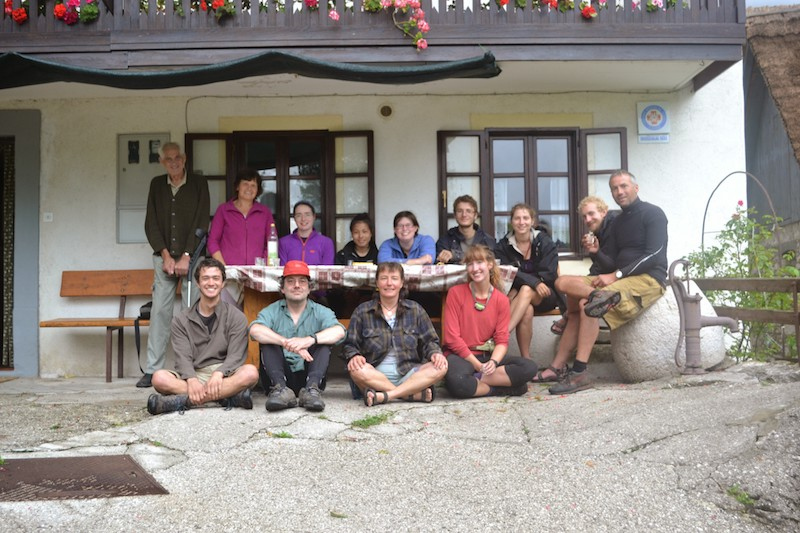
\includegraphics[width=0.99\textwidth]{images/2014/other-finds-2014/end_of_expo_2014.jpg}}
\caption{The team at the end of expedition Skosi Zrcalo 2014  \emph{back left to right} Marjan Koblucar, Slavica Koblucar, Aileen Brown, Sarah Gian, Fiona Hartley, Tanguy Racine, Nadine Kalmoni, Dave Kirkpatrick \emph{front left to right} Rhys Tyers, Dave Wilson, Janet Cotter, Kate Smith, James 'Tetley' Hooper}
\label{end of expo 2}
\end{pagefigure}

\clearpage


 \begin{figure*}
 \centering
 \begin{tikzpicture}
\node [table] (box){%
    \begin{minipage}{\textwidth}
\centering
    \begin{tabular}{lrrrr}
    Sector & \multicolumn{1}{l}{Passage name} & Survey length (m) & Stations & Average leg (m) \\ \midrule
    \multirow{6}[0]{*}{Atlantis} & \multicolumn{1}{l}{Jericho} & 80.87 & 12    & 7.35 \\
          & \multicolumn{1}{l}{Jericho2} & 40.56 & 9     & 5.07 \\
          & \multicolumn{1}{l}{Pleasure Palace} & 93.36 & 21    & 4.67 \\
          & \multicolumn{1}{l}{Sic Semper Tyrannis} & 177.05 & 28    & 6.56 \\
          & \multicolumn{1}{l}{Squidgy Goodness} & 28.87 & 9     & 3.61 \\
          & \multicolumn{1}{l}{Touching the Void} & 79.86 & 6     & 15.97 \\ \midrule
    \multirow{3}[0]{*}{Balamory} & \multicolumn{1}{l}{Aja?!} & 167.7 & 31    & 5.59 \\
          & \multicolumn{1}{l}{Hanging Gardens (deep)} & 55.84 & 13    & 4.65 \\
          & \multicolumn{1}{l}{Rock Steady Love} & 96.95 & 16    & 6.46 \\ \midrule
    \multirow{2}[0]{*}{Esoterica} & \multicolumn{1}{l}{Serrure} & 78.87 & 18    & 4.64 \\
          & \multicolumn{1}{l}{Your Mum} & 11.67 & 5     & 2.92 \\ \midrule
    \multirow{3}[0]{*}{Kamikaze} & \multicolumn{1}{l}{A Pun Too Far 1} & 36.6  & 12    & 3.33 \\
          & \multicolumn{1}{l}{A Pun Too Far 2} & 26.84 & 10    & 2.98 \\
          & \multicolumn{1}{l}{A Pun Too Far 3} & 80.64 & 17    & 5.04 \\ \midrule
    \multirow{3}[0]{*}{Xanadu} & \multicolumn{1}{l}{Gravity} & 123.57 & 29    & 4.41 \\
          & \multicolumn{1}{l}{Hips Don't Lie} & 19.33 & 10    & 2.15 \\
          & \multicolumn{1}{l}{Stupid} & 7.5   & 4     & 2.50 \\ \midrule
          &       &       &       &  \\
    \textbf{Total} &       & \textbf{1206.08} &       &  \\
    \end{tabular}%
  \label{tab:addlabel}%
  \end{minipage}
  };
\node[tabletitle, right=10pt] at (box.north west) {Number crunching};
\end{tikzpicture}
\end{figure*}

%__________________


\begin{figure*}[t!]
\centering
\frame{\includegraphics[width=\textheight, angle=270]{"images/2014/other-finds-2014/2014plan".pdf}}
\caption{}
\label{}
\end{figure*}

\begin{figure*}[t!]
\centering
\frame{\includegraphics[height=\textheight]{"images/2014/other-finds-2014/ee2014".pdf}}
\caption{}
\label{}
\end{figure*}